% Asal-usul (tidak pernah dicetak): lihat sources/outline_sources.md (Tahun 1: pembagian litostratigrafi, biostratigrafi dan kronostratigrafi; batas stratotipe; kepunahan massal sebagai penanda global; bagan internasional). Nilai soal latihan dan soal dalam kalkulator skrap Buku 3 calc/ch24.py; bagan dari figdata/bachelor-1/ics_chart.py (baris ics bersama). Prinsip penentuan umur relatif, era dan periode milik Buku 1 (kelas 7, waktu geologi) dan didirikan ulang di sini. Kepunahan massal milik seri biologi (diingat kembali dalam prosa); penyebab-penyebab di Bumi milik volume Tahun ke-2 (fanerozoikum Bumi). Korelasi log dan ketidakselarasan milik bab 5; fasies milik bab 21; pemadatan milik bab 23. Penanggalan radiometrik milik bab 25. Stratigrafi urutan, model fasies dan hukum Walther adalah milik volume Tahun ke-3; magnetostratigrafi juga: hanya penunjuk prosa. "Transgresi" dijelaskan dalam prosa.
\chapter{Skala stratigrafi}\label{ch:b1:stratigraphic-scale}

Di pantai Itzurun, di Zumaia di pantai Basque, tebing-tebingnya tersusun dari lapisan tipis batu kapur dan marl, miring dan berulang sepanjang ratusan meter. Di satu \omterm{def:b1:geological-maps:geological-map}{kontak}, tempat lapisan batu kapur pucat berakhir dan marl merah mulai, sebuah cakram perunggu yang dicap dengan empat huruf ditanamkan ke dalam batuan (gambar di bawah). Itu adalah paku emas. Ia menetapkan, untuk seluruh planet, saat ketika satu pembagian waktu geologi --- \omterm{def:b1:stratigraphic-scale:chronostratigraphy}{Tahap} Selandian --- dimulai. Batuan di Patagonia atau di Siberia termasuk Selandian jika ia diendapkan setelah saat yang tercatat di \omterm{def:b1:geological-maps:geological-map}{kontak} itu dan sebelum saat yang tercatat pada paku berikutnya di atas skala. Bab ini menjelaskan bagaimana geolog memerlukan penanda semacam itu: tiga cara berbeda membagi tumpukan batuan, prinsip-prinsip yang mengurutkannya, garis-garis yang menghubungkan penampang yang berjauhan, dan bagan internasional yang menghimpun hasilnya.

\begin{omfigure}
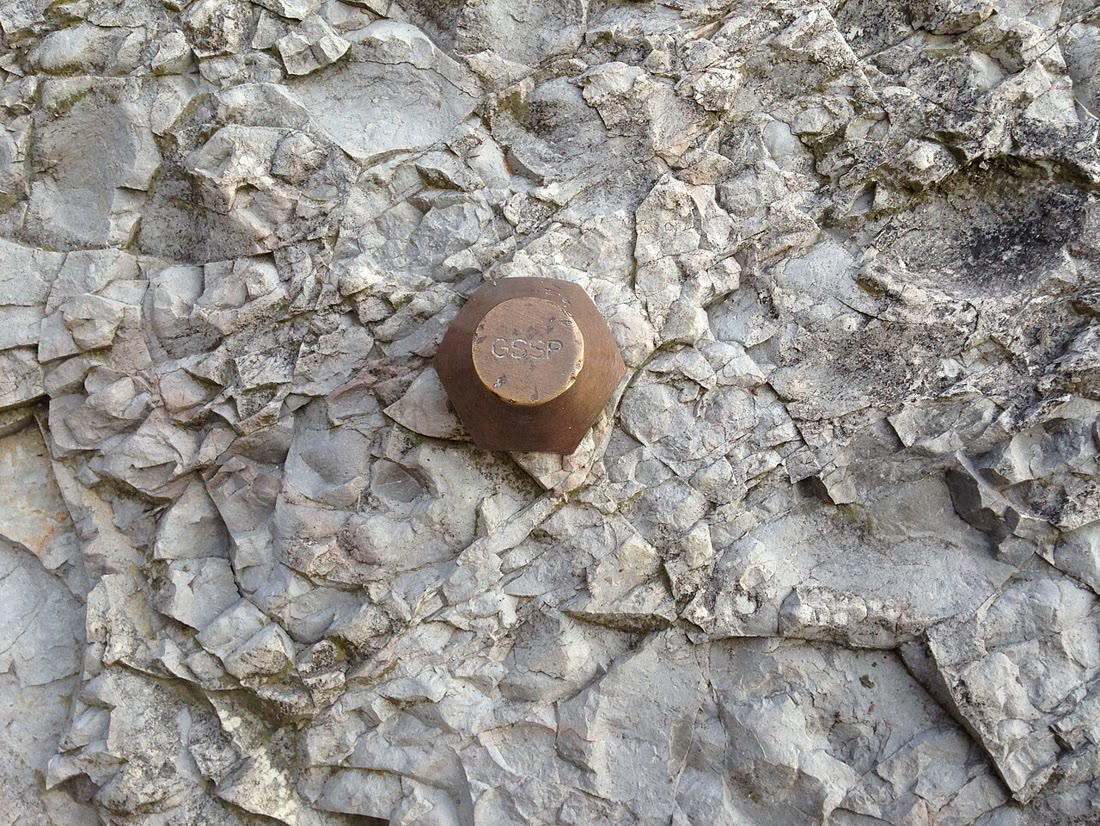
\includegraphics[width=0.62\linewidth]{images/book3/b1-golden-spike-zumaia.jpg}

{\small Penanda emas \omterm{def:b1:stratigraphic-scale:chronostratigraphy}{Tahap} Selandian di penampang Zumaia: penanda perunggu yang dicap GSSP, dipasang di puncak lapisan batu kapur tertinggi suatu \omterm{def:b1:stratigraphic-scale:lithostratigraphy}{formasi}, di dasar marl merah \omterm{def:b1:stratigraphic-scale:lithostratigraphy}{formasi} berikutnya. (Josugoni, CC~BY-SA~4.0, melalui Wikimedia Commons.)}
\label{fig:b1:stratigraphic-scale:zumaia}
\end{omfigure}
% ledger: commons:zumaia-gssp, gssp:selandian

\begin{recall}
Dalam tumpukan lapisan yang belum terbalik, setiap lapisan lebih muda daripada yang di bawahnya; struktur yang memotong batuan lebih muda daripada batuan itu; fosil berubah dari lapisan yang lebih tua ke yang lebih muda dengan urutan yang sama di mana-mana; sejarah Bumi dibagi menjadi era dan periode geologi, masing-masing dengan umur dalam tahun untuk awalnya, yang dihimpun dalam bagan internasional (Buku~1, kelas~7). \omterm{def:b1:cross-sections:log}{Log lubang bor} mencatat satuan yang ditemui terhadap kedalaman, dan korelasi mencocokkan satuan yang sama dari log ke log (\cref{def:b1:cross-sections:log}); \omterm{def:b1:cross-sections:unconformity}{ketidakselarasan} adalah permukaan erosi atau non-pengendapan (\cref{def:b1:cross-sections:unconformity}). \omterm{def:b1:clastic-sediments:facies}{Fasies sedimen} adalah sebuah tubuh batuan yang karakternya mencatat \omterm{def:b1:clastic-sediments:facies}{lingkungan pengendapannya} (\cref{def:b1:clastic-sediments:facies}). Volume biologi menjelaskan bagaimana spesies muncul dan punah, dan beberapa kepunahan massal tempat sebagian besar spesies hilang dalam waktu singkat.
\end{recall}

\section{Tiga cara membagi batuan}\label{sec:b1:stratigraphic-scale:three}

Seorang geolog yang mencatat sebuah tebing dapat membagi tumpukan lapisan yang sama dengan tiga cara: menurut apa yang dibuat oleh batuan, menurut fosil yang dikandungnya, dan menurut waktu tempat ia diendapkan. Ketiga pembagian itu menjawab pertanyaan yang berbeda, dan batasnya tidak harus berimpit. Aturan penamaan dan pendefinisian setiap jenis satuan ditetapkan oleh kesepakatan internasional.
% ledger: isg:lithostratigraphy

\begin{definition}[Formasi, anggota, grup]\label{def:b1:stratigraphic-scale:lithostratigraphy}
Sebuah \emph{satuan litostratigrafi}\index{satuan litostratigrafi} adalah sebuah tubuh batuan yang didefinisikan dan dikenali oleh litologinya dan posisinya di antara tubuh-tubuh lain, apa pun umurnya. Satuan utamanya adalah \emph{formasi}\index{formasi (litostratigrafi)}: sebuah tubuh batuan yang cukup berbeda dari tetangganya untuk dipetakan pada skala wilayah, ke dalam mana seluruh kolom sebaiknya dibagi. Sebuah \emph{anggota}\index{anggota (litostratigrafi)} adalah subdivisi bernama dari sebuah formasi, dibedakan oleh litologinya; sebuah \emph{grup}\index{grup (litostratigrafi)} adalah suksesi dua formasi atau lebih yang memiliki karakter litologi yang signifikan bersama. Sebuah nama formal menggabungkan nama geografis setempat dengan peringkat atau batuan dominan: Batu Pasir Kell, Formasi Serpih Mardon.
\end{definition}
% ledger: isg:lithostratigraphy

Sebuah \omterm{def:b1:stratigraphic-scale:lithostratigraphy}{formasi} dapat setebal kurang dari satu meter atau beberapa ribu meter. Ia diperluas jauh dari penampang tipenya hanya sejauh litologinya dapat dikenali, sehingga batas-batasnya mengikuti batuan, bukan waktu.
% ledger: isg:lithostratigraphy

\begin{definition}[Biozona, fosil indeks, datum kemunculan pertama]\label{def:b1:stratigraphic-scale:biozone}
Sebuah \emph{biozona}\index{biozona} adalah tubuh lapisan yang didefinisikan atau dicirikan oleh fosil yang dikandungnya. Sebuah \emph{zona rentang}\index{zona rentang} memuat kemunculan yang diketahui dari satu takson; sebuah \emph{zona interval}\index{zona interval} adalah tubuh lapisan di antara dua horizon fosil yang ditentukan, misalnya kemunculan terendah dari dua takson. \emph{Datum kemunculan pertama}\index{datum kemunculan pertama} (FAD) dari suatu takson adalah horizon kemunculan terendahnya, \emph{datum kemunculan terakhir}\index{datum kemunculan terakhir} adalah yang tertingginya. Sebuah \emph{fosil indeks}\index{fosil indeks} adalah takson yang digunakan untuk mengenali sebuah biozona: yang terbaik tersebar luas, melimpah, mudah diidentifikasi dan berumur pendek.
\end{definition}
% ledger: isg:biostratigraphy, og:stratigraphy-principles

Horizon fosil tidak memiliki ketebalan; sebuah \omterm{def:b1:stratigraphic-scale:biozone}{biozona} dapat setebal beberapa meter atau beberapa ratus meter, bergantung pada seberapa cepat sedimen terakumulasi selama takson itu hidup. Karena spesies berevolusi dan tidak pernah muncul kembali setelah punah, kumpulan fosil dari satu umur tertentu bersifat unik. Beberapa \omterm{def:b1:stratigraphic-scale:biozone}{fosil indeks} terbaik adalah mikrofosil, seperti foraminifera dan konodont: tersebar luas, melimpah, dan cukup kecil untuk diambil dari serpihan sebuah sumur.
% ledger: isg:biostratigraphy, og:stratigraphy-principles

\begin{definition}[Satuan kronostratigrafi dan geokronologi]\label{def:b1:stratigraphic-scale:chronostratigraphy}
Sebuah \emph{satuan kronostratigrafi}\index{satuan kronostratigrafi} adalah tubuh seluruh batuan yang terbentuk selama interval waktu geologi tertentu, dan hanya selama itu; batas-batasnya adalah permukaan dengan umur yang sama. Interval waktu itu sendiri adalah sebuah \emph{satuan geokronologi}\index{satuan geokronologi}. Peringkat-peringkatnya, dari yang terkecil, adalah \emph{tahap}\index{tahap (kronostratigrafi)} (waktunya: sebuah umur), \emph{seri}\index{seri (kronostratigrafi)} (sebuah epok), dan
\emph{sistem}\index{sistem (kronostratigrafi)} (sebuah periode), eratem (sebuah era) dan eonotem (sebuah eon); setiap satuan tersusun dari beberapa satuan berurutan dari peringkat di bawahnya.
\end{definition}
% ledger: isg:chronostratigraphy

Kedua kata itu menggambarkan pembagian yang sama dilihat sebagai batuan atau sebagai waktu (\cref{tab:b1:stratigraphic-scale:ranks}): batuan \omterm{def:b1:stratigraphic-scale:chronostratigraphy}{Sistem} Jura diendapkan selama Periode Jura, dan \omterm{def:b1:stratigraphic-scale:chronostratigraphy}{Seri} Jura Bawah selama Epok Jura Awal. \omterm{def:b1:stratigraphic-scale:chronostratigraphy}{Tahap} adalah satuan terkecil yang dikenali di seluruh dunia.
% ledger: isg:chronostratigraphy, chart:danian

\begin{table}[htbp]
\centering
{\setlength{\tabcolsep}{4pt}\begin{tabular}{lll}
\hline
\omterm{def:b1:stratigraphic-scale:chronostratigraphy}{satuan kronostratigrafi} (batuan) & \omterm{def:b1:stratigraphic-scale:chronostratigraphy}{satuan geokronologi} (waktu) & contoh \\
\hline
eonotem & eon    & Fanerozoikum \\
eratem   & era    & Kenozoikum \\
\omterm{def:b1:stratigraphic-scale:chronostratigraphy}{sistem}   & periode & Paleogen \\
\omterm{def:b1:stratigraphic-scale:chronostratigraphy}{seri}   & epok  & Paleosen \\
\omterm{def:b1:stratigraphic-scale:chronostratigraphy}{tahap}    & umur   & Danian (\qtyrange{66.00}{61.66}{\Ma}) \\
\hline
\end{tabular}}
\caption{Peringkat \omterm{def:b1:stratigraphic-scale:chronostratigraphy}{satuan kronostratigrafi} dan geokronologi, dengan satuan-satuan yang memuat Danian, \omterm{def:b1:stratigraphic-scale:chronostratigraphy}{tahap} pertama Kenozoikum.}
\label{tab:b1:stratigraphic-scale:ranks}
\end{table}
% ledger: isg:chronostratigraphy, chart:danian

\section{Prinsip dan korelasi}\label{sec:b1:stratigraphic-scale:principles}

Sebelum batuan mana pun dapat ditanggal dalam tahun, urutan peristiwa dibaca dari batuan itu sendiri. Prinsip-prinsip dasar stratigrafi dikemukakan pada 1669 oleh Nicolas Steno; antara 1785 dan 1800 Hutton dan William Smith menambahkan pemakaian lapisan sebagai interval waktu dan fosilnya untuk mengenalinya.
% ledger: og:stratigraphy-principles, usgs:hutton-smith

\begin{definition}[Prinsip-prinsip stratigrafi]\label{def:b1:stratigraphic-scale:principles}
\begin{enumerate}
  \item \emph{Prinsip superposisi}\index{superposisi, prinsip}: dalam suatu urutan lapisan sedimen yang belum terbalik, setiap lapisan lebih muda daripada lapisan tempat ia bertumpu.
  \item \emph{Prinsip horizontalitas asal}\index{horizontalitas asal, prinsip}: sedimen dan aliran lava diendapkan secara mendatar, atau hampir demikian --- sedikit miring di tepi cekungan.
  \item \emph{Prinsip kontinuitas lateral}\index{kontinuitas lateral, prinsip}: di dalam sebuah cekungan, sebuah lapisan memanjang secara kontinu ke segala arah hingga menipis di tepi cekungan atau di hadapan halangan; lapisan yang terpotong oleh lembah berlanjut di sisi lain.
  \item \emph{Prinsip hubungan memotong}\index{hubungan memotong, prinsip}: sebuah tubuh atau struktur yang memotong batuan --- sebuah dike, sesar, permukaan erosi --- lebih muda daripada batuan yang dipotongnya.
  \item \emph{Prinsip suksesi fauna}\index{suksesi fauna, prinsip}: takson fosil bergantian satu sama lain dengan urutan yang sama di setiap wilayah, sehingga batuan yang memuat kumpulan yang sama berumur sama.
\end{enumerate}
\end{definition}
% ledger: og:stratigraphy-principles, eli:relative-dating, usgs:fossil-succession, isg:chronostratigraphy

Prinsip-prinsip itu tidak sama kuatnya. Superposisi memberi urutan yang harus dihormati oleh setiap metode lain. Horizontalitas asal adalah yang membuat lapisan yang miring menjadi catatan deformasi kemudian. Kontinuitas lateral adalah yang memungkinkan geolog menggambar lapisan yang sama di kedua sisi lembah, dan, dalam jarak terbatas, bidang perlapisan yang ditelusuri di lapangan adalah garis berumur sama terbaik yang ada. Suksesi fauna adalah yang melintasi samudra; ia menjadi pokok bahasan paragraf-paragraf berikutnya.
% ledger: isg:chronostratigraphy, og:stratigraphy-principles

\subsection*{Korelasi dengan biozona}

\omterm{def:b1:cross-sections:log}{Korelasi} dengan fosil membandingkan urutan kemunculan dan kepunahan pertama dan terakhir di dua penampang (gambar di bawah). Keduanya tidak sama andal. Fosil tertinggi dari suatu takson yang ditemukan di sebuah penampang bergantung pada berapa banyak yang terawetkan: di tempat yang jarang, fosil terakhir yang ditemukan mungkin terletak jauh di bawah tingkat tempat takson itu benar-benar punah, dan fosil yang tererosi dan diendapkan kembali dapat muncul di atasnya. Kemunculan pertama juga dapat bergeser, tetapi takson yang tersebar luas dan menyebar cepat dicapai pada tingkat yang kurang lebih sama di seluruh cekungan.
% ledger: isg:biostratigraphy

\begin{omfigure}
\begin{tikzpicture}[font=\footnotesize, y=0.13cm]
  % section 1: 40 m, sandstone 0-14, shale 14-40
  \fill[lith sandstone] (0,0) rectangle (0.8,14);
  \fill[lith shale] (0,14) rectangle (0.8,40);
  \draw[black!70] (0,0) rectangle (0.8,40);
  \node[anchor=south, font=\small] at (1.4,41.5) {penampang 1};
  \foreach \x/\a/\b/\t in {1.1/0/27/a, 1.4/10/34/b, 1.7/20/40/c, 2.0/30/40/d} {
    \draw[line width=2.2pt, omThm] (\x,\a) -- (\x,\b);
    \node[anchor=base, font=\scriptsize] at (\x,-4.5) {\t};
  }
  \foreach \y/\z in {5/a, 15/b, 25/c, 35/d}
    \node[anchor=east, font=\scriptsize] at (-0.1,\y) {zona \z};
  \foreach \y in {10,20,30} \draw[black!50] (-1.3,\y) -- (0,\y);
  % scale bar
  \draw[thick] (-1.5,0) -- (-1.5,10) node[midway, anchor=east, font=\scriptsize] {\qty{10}{m}};
  % section 2: 24 m, sandstone 0-3, shale 3-24
  \begin{scope}[xshift=7cm]
    \fill[lith sandstone] (0,0) rectangle (0.8,3);
    \fill[lith shale] (0,3) rectangle (0.8,24);
    \draw[black!70] (0,0) rectangle (0.8,24);
    \node[anchor=south, font=\small] at (1.4,25.5) {penampang 2};
    \foreach \x/\a/\b/\t in {1.1/0/13/a, 1.4/6/20/b, 1.7/12/24/c, 2.0/18/24/d} {
      \draw[line width=2.2pt, omThm] (\x,\a) -- (\x,\b);
      \node[anchor=base, font=\scriptsize] at (\x,-4.5) {\t};
    }
    \foreach \y/\z in {3/a, 9/b, 15/c, 21/d}
      \node[anchor=west, font=\scriptsize] at (2.3,\y) {zona \z};
    \foreach \y in {6,12,18} \draw[black!50] (0.8,\y) -- (2.3,\y);
  \end{scope}
  % correlation of the first appearances
  \foreach \u/\v/\t in {10/6/b, 20/12/c, 30/18/d}
    \draw[densely dashed, omThm!70!black] (2.15,\u) -- (6.85,\v)
      node[pos=0.5, fill=white, inner sep=1pt, font=\scriptsize] {FAD \t};
\end{tikzpicture}

{\small Diagram rentang dan korelasi dengan \omterm{def:b1:stratigraphic-scale:biozone}{biozona} (takson rekaan \emph{a} hingga \emph{d}). Batang tebal adalah rentang takson di setiap penampang. Tiga \omterm{def:b1:stratigraphic-scale:biozone}{zona interval} dibatasi oleh kemunculan pertama \emph{b}, \emph{c} dan \emph{d}, yang disambungkan dari penampang ke penampang (putus-putus). Kemunculan terakhir \emph{a} jatuh di bagian atas zona~\emph{c} di penampang 1 dan dekat dasarnya di penampang 2: ia adalah panduan yang lebih buruk. Zona-zona lebih tipis di penampang 2, tempat sedimen terakumulasi lebih lambat.}
\label{fig:b1:stratigraphic-scale:range-chart}
\end{omfigure}

\begin{method}[Mengorelasikan penampang dengan biozona]\label{met:b1:stratigraphic-scale:biozones}
\begin{enumerate}
  \item Plot, untuk setiap penampang, rentang setiap takson terhadap ketinggian: dari kemunculan terendah hingga tertingginya.
  \item Pilih horizon fosil yang mendefinisikan zona --- sebaiknya kemunculan pertama takson yang tersebar luas dan tidak bergantung pada fasies.
  \item Gambar batas zona di setiap penampang pada horizon-horizon ini.
  \item Sambungkan horizon yang sama dari penampang ke penampang; periksa bahwa garis-garisnya tidak bersilangan, seperti yang dituntut superposisi.
  \item Bacalah, di antara dua garis, ketebalan setiap zona di setiap penampang; di tempat suatu zona hilang, carilah \omterm{def:b1:cross-sections:unconformity}{ketidakselarasan} atau perubahan fasies sebelum menyimpulkan bahwa takson itu tidak ada.
\end{enumerate}
\end{method}

Sebuah \omterm{def:b1:stratigraphic-scale:biozone}{biozona} hanya sebaik kebebasan fosilnya dari lingkungan. Kerang yang hidup hanya di pantai berpasir hanya ditemukan di batu pasir; mengikutinya dari penampang ke penampang berarti mengikuti batu pasir, bukan waktu. \omterm{def:b1:cross-sections:log}{Korelasi} biostratigrafi karena itu belum tentu korelasi waktu: ia dapat mengikuti fasies yang umurnya berubah dari tempat ke tempat.
% ledger: isg:biostratigraphy

\subsection*{Batas-batas yang melintasi waktu}

Sedimen yang berbeda diendapkan pada waktu yang sama di tempat yang berbeda: pasir di pantai, lumpur di lepas pantai, kapur lebih jauh di paparan yang kekurangan pasir. Garis berumur sama karena itu melintasi dari satu litologi ke litologi lain. Sebaliknya, batas litologi yang ditelusuri di seluruh cekungan belum tentu merupakan garis berumur sama sepenuhnya.
% ledger: og:stratigraphy-principles, isg:chronostratigraphy

\begin{definition}[Batas diakronis]\label{def:b1:stratigraphic-scale:diachronous}
Sebuah batas bersifat \emph{diakronis}\index{batas diakronis} ketika umurnya berubah dari tempat ke tempat sepanjangnya. Batas \omterm{def:b1:stratigraphic-scale:lithostratigraphy}{formasi} dan fasies umumnya diakronis; batas \omterm{def:b1:stratigraphic-scale:chronostratigraphy}{satuan kronostratigrafi}, menurut definisi, tidak.
\end{definition}
% ledger: isg:lithostratigraphy, isg:chronostratigraphy, isg:biostratigraphy

Kasus klasiknya adalah transgresi: \omterm{def:b1:diagenesis-basins:eustasy}{muka laut relatif} naik lebih cepat daripada sedimen dapat mengisi ruang yang tercipta, dan garis pantai bergerak ke daratan. Pasir pantai diendapkan di garis pantai setiap saat, sehingga selembar batu pasir menyebar ke daratan bersamanya; lumpur lepas pantai menyusul di atasnya. Puncak batu pasir kemudian menjadi jejak garis pantai yang bergerak: muda di daratan, tua ke arah laut (gambar di bawah). Urutan fasies yang terlihat dalam satu penampang vertikal --- batu pasir di bawah serpih di bawah batu kapur --- mengulang urutannya di seluruh paparan pada satu saat; volume Tahun ke-3 menjadikan ini dasar model fasiesnya.
% ledger: og:stratigraphy-principles, isg:lithostratigraphy

\begin{omfigure}
\begin{tikzpicture}[font=\footnotesize, x=1cm, y=1cm]
  % basement surface B(x) = 1.6 (1 - x/14), rising towards the land on the left
  \fill[lith granite] (0,-0.5) -- (0,1.6) -- (14,0) -- (14,-0.5) -- cycle;
  \fill[lith sandstone] (0,1.6) -- (14,0) -- (14,0.5) -- (0,2.1) -- cycle;
  \fill[lith shale] (0,2.1) -- (14,0.5) -- (14,1.5) -- (0,3.1) -- cycle;
  \fill[lith limestone] (0,3.1) -- (14,1.5) -- (14,3.6) -- (0,3.6) -- cycle;
  \draw[unconformity] (0,1.6) -- (14,0);
  \draw[black!70] (0,2.1) -- (14,0.5) (0,3.1) -- (14,1.5);
  \draw[black!70] (0,-0.5) rectangle (14,3.6);
  % time lines: horizontal, from the basement (or the left edge) to the right edge
  \foreach \y/\t in {0.6/1, 1.1/2, 1.6/3, 2.1/4, 2.6/5, 3.1/6} {
    \pgfmathsetmacro{\xs}{max(0, 14*(1-\y/1.6))}
    \draw[omThm, thick, densely dashed] (\xs,\y) -- (14,\y) node[anchor=west, text=black] {$t_\t$};
  }
  % two sections
  \foreach \x/\n in {3/1, 11/2} {
    \draw[very thick, black] (\x,-0.5) -- (\x,3.6);
    \node[anchor=south, font=\small] at (\x,3.65) {penampang \n};
  }
  \node[fill=white, inner sep=1pt, font=\scriptsize] at (5.6,1.21) {batu pasir};
  \node[fill=white, inner sep=1pt] at (12.6,1.2) {serpih};
  \node[fill=white, inner sep=1pt] at (7.0,3.25) {batu kapur};
  \node[fill=white, inner sep=1pt] at (12.0,-0.25) {batuan dasar};
  \draw[-{Stealth}, thick] (5.6,4.35) -- (3.6,4.35) node[anchor=east] {darat};
  \draw[-{Stealth}, thick] (8.4,4.35) -- (10.4,4.35) node[anchor=west] {laut};
\end{tikzpicture}

{\small Batu pasir yang diendapkan selama transgresi (skematis, skala vertikal dilebih-lebihkan). Garis putus-putus $t_1$ hingga $t_6$ menghubungkan titik-titik berumur sama, $t_1$ yang tertua. Di tempat satu garis bertemu batuan dasar, ia dimulai di garis pantai pada waktunya; ke arah laut ia berubah dari pasir menjadi lumpur dan, pada yang lebih muda, menjadi kapur. Puncak batu pasir terletak di antara $t_1$ dan $t_2$ pada penampang 2 tetapi di antara $t_3$ dan $t_4$ pada penampang 1: batas \omterm{def:b1:stratigraphic-scale:lithostratigraphy}{formasi} itu \omterm{def:b1:stratigraphic-scale:diachronous}{diakronis}, makin muda ke arah daratan.}
\label{fig:b1:stratigraphic-scale:diachronous}
\end{omfigure}

Seberapa cepat umur batas itu berubah di sepanjangnya? Pada dataran pantai yang naik landai ke pedalaman, jawabannya adalah soal geometri.

\begin{proposition}[Kecepatan transgresi]\label{prop:b1:stratigraphic-scale:transgression}
Sebuah dataran pantai naik ke arah pedalaman dengan gradien seragam $s$, dan \omterm{def:b1:diagenesis-basins:eustasy}{muka laut relatif} naik dengan laju tetap $R$, tanpa sedimen yang ditambahkan di pantai. Garis pantai kemudian bergerak ke pedalaman dengan kecepatan
\[
  u = \frac{R}{s},
\]
dan sebuah batas yang mengikuti garis pantai lebih muda, di suatu titik berjarak $d$ lebih jauh ke pedalaman, sebesar $\Delta t = d/u = d\,s/R$.
\end{proposition}

\begin{proof}
Ambil $x$ sebagai jarak ke pedalaman dari suatu titik tetap dan $z$ sebagai tinggi; dataran adalah garis $z = s x$, dan permukaan laut pada waktu $t$ adalah
$z = z_0 + R t$. Garis pantai adalah tempat keduanya bertemu: $s\,x(t) = z_0 + R t$, sehingga
$x(t) = (z_0 + R t)/s$ dan $\mathrm dx/\mathrm dt = R/s$. Garis pantai mencapai sebuah titik berjarak $d$ lebih jauh ke pedalaman setelah waktu $d/u = d\,s/R$.
\end{proof}

Rasionya besar karena dataran pantai hampir datar. Kenaikan \qty{10}{m} per juta tahun di atas dataran yang miring $1$ banding $2000$ memindahkan pantai \qty{20}{km} ke pedalaman per juta tahun; puncak batu pasir yang tampak seperti satu permukaan di tebing kemudian berumur satu juta tahun lebih muda pada jarak \qty{20}{km} ke pedalaman. Sedimen yang dibawa ke pantai memperlambat transgresi atau membalikkannya.

\subsection*{Garis berumur sama}

Apa yang mengkorelasikan waktu, kalau begitu, jika litologi tidak, dan fosil hanya kira-kira? Garis yang terbaik dibuat oleh peristiwa yang meninggalkan jejak di mana-mana sekaligus. Abu vulkanik jatuh di wilayah yang luas dalam apa yang, secara geologi, merupakan sekejap, dan mengendap di atas pasir, lumpur dan kapur sama saja: lapisan abu adalah garis berumur sama yang melintasi batas fasies, dan sering dapat ditanggal dalam tahun dengan metode dalam \cref{ch:b1:radiometric-methods}. Pembalikan medan magnet Bumi, yang dibahas dalam volume Tahun ke-3, tercatat dalam batuan dari banyak jenis dan dapat dikenali di seluruh dunia setelah urutannya diketahui; demikian pula pergeseran tajam pada isotop karbon, seperti yang menandai dasar Ypresian (\cref{tab:b1:stratigraphic-scale:gssps}). Di antara dua level yang bertarikh, umur lapisan mana pun diperkirakan dengan mengasumsikan bahwa sedimen terakumulasi pada laju tetap.
% ledger: isg:chronostratigraphy

\begin{proposition}[Umur di antara dua level bertarikh]\label{prop:b1:stratigraphic-scale:interpolation}
Dua lapisan pada ketinggian $z_1 < z_2$ dari suatu penampang kontinu memiliki umur $t_1 > t_2$. Jika sedimen terakumulasi pada laju tetap di antara keduanya, sebuah level pada ketinggian $z$ di antaranya memiliki umur
\[
  t = t_1 - f\,(t_1 - t_2), \qquad f = \frac{z - z_1}{z_2 - z_1},
\]
dan laju akumulasinya adalah $r = (z_2 - z_1)/(t_1 - t_2)$. Jika kedua umur membawa ketidakpastian baku yang independen $\sigma_1$ dan $\sigma_2$, umur yang diinterpolasi membawa ketidakpastian
\[
  \sigma_t = \sqrt{(1 - f)^2 \sigma_1^2 + f^2 \sigma_2^2}.
\]
\end{proposition}

\begin{proof}
Pada laju konstan $r$, tinggi tumbuh secara linier terhadap waktu: $z - z_1 = r\,(t_1
- t)$, karena umur berkurang ke atas. Di $z_2$, $z_2 - z_1 = r\,(t_1 - t_2)$, yang memberi $r$; membagi kedua hubungan memberi $t_1 - t = f\,(t_1 - t_2)$. Umur adalah kombinasi linear $t = (1 - f)\,t_1 + f\,t_2$ dari dua besaran yang independen; varians $a X + b Y$ untuk $X$ dan $Y$ yang independen adalah $a^2
\operatorname{Var} X + b^2 \operatorname{Var} Y$, yang memberi $\sigma_t$.
\end{proof}

Ketidakpastiannya paling kecil di antara kedua lapisan bertarikh dan tidak pernah lebih besar daripada yang lebih besar dari $\sigma_1$ dan $\sigma_2$ di sana. Batas sebenarnya adalah asumsinya: sedimen terakumulasi dalam denyut, dapat berhenti di celah tersembunyi, dan memadat secara berbeda di pasir dan di lumpur (\cref{prop:b1:diagenesis-basins:solid}), sehingga umur yang diinterpolasi tidak lebih baik daripada keteraturan penampang.

\section{Stratotipe batas}\label{sec:b1:stratigraphic-scale:gssp}

\omterm{def:b1:stratigraphic-scale:chronostratigraphy}{Satuan kronostratigrafi} didefinisikan dalam batuan sebelum ditanggal. Praktik lama menjelaskan setiap \omterm{def:b1:stratigraphic-scale:chronostratigraphy}{tahap} dengan sebuah penampang tipe dari seluruh satuan; tetapi puncak satu penampang tipe dan dasar yang berikutnya, dipilih di tempat yang berbeda, dapat meninggalkan celah waktu tak bertugas di antara keduanya atau tumpang tindih. Praktik modern hanya mendefinisikan batas bawah setiap satuan di satu titik dalam satu penampang; batas atasnya adalah batas bawah satuan berikutnya. Tidak ada interval waktu kemudian yang dapat jatuh di antara dua satuan atau termasuk dalam keduanya.
% ledger: isg:stratotype, isg:chronostratigraphy

\begin{definition}[Stratotipe batas, stratotipe satuan, GSSP]\label{def:b1:stratigraphic-scale:gssp}
Sebuah \emph{stratotipe}\index{stratotipe} adalah penampang batuan yang ditunjuk yang berfungsi sebagai standar acuan untuk sebuah satuan atau batas. Sebuah \emph{stratotipe satuan}\index{stratotipe satuan} adalah penampang tipe dari seluruh satuan; sebuah \emph{stratotipe batas}\index{stratotipe batas} adalah penampang yang memuat titik spesifik yang mendefinisikan batas antara dua satuan. Sebuah \emph{penampang dan titik stratotipe batas global}\index{penampang dan titik stratotipe batas global (GSSP)} (GSSP) adalah stratotipe batas dari sebuah satuan skala kronostratigrafi internasional: sebuah titik tunggal dalam satu penampang, dipilih menurut kesepakatan internasional, yang mendefinisikan dasar sebuah \omterm{def:b1:stratigraphic-scale:chronostratigraphy}{tahap} dan setiap satuan yang lebih besar yang dimulai dengannya.
\end{definition}
% ledger: isg:stratotype, isg:chronostratigraphy, gssp:protocol

GSSP adalah titik dalam batuan, bukan umur. Umurnya dalam tahun adalah apa pun yang diberikan oleh penanggalan terbaik titik itu, dan ia dapat diperhalus tanpa memindahkan titik. Penampang dipilih agar titik itu dapat ditemukan kembali di tempat lain: pengendapan menerus di seluruh batas (tidak pernah pada \omterm{def:b1:cross-sections:unconformity}{ketidakselarasan}, tempat waktu yang hilang akan membuat batas itu ambigu), sebaiknya laut, kaya fosil terawetkan dengan baik dari takson yang tersebar luas, tanpa perubahan fasies pada level itu, sedikit terdeformasi atau terubah, mudah diakses dan terlindungi. Yang terpenting, titik itu ditempatkan pada level yang berimpit dengan satu sinyal yang dipilih --- biasanya kemunculan pertama suatu takson --- di dalam interval yang kaya akan sinyal lain (lapisan abu, pembalikan magnetik, pergeseran isotop) yang dengannya level itu dapat dikenali dari jauh. Penanda permanen, paku emas, dipasang di titik itu.
% ledger: isg:chronostratigraphy, isg:stratotype, gssp:protocol

\begin{inthefield}[Bagaimana sebuah batas dipilih]
Sebuah batas dipelajari oleh kelompok kerja subkomisi yang bertanggung jawab atas \omterm{def:b1:stratigraphic-scale:chronostratigraphy}{sistem}, yang membandingkan penampang-penampang calon, mencatat logs-nya lapis demi lapis, mengambil sampel fosilnya, lapisan abu dan isotopnya, dan menulis usulan. Sebuah usulan memerlukan mayoritas super --- lebih dari \qty{60}{\%} --- dari anggota pemberi suara subkomisi, sekitar dua puluh spesialis; lalu ia diteruskan kepada anggota pemberi suara Komisi Stratigrafi Internasional, para pejabat eksekutif dan ketua tujuh belas subkomisinya, dan akhirnya kepada komite eksekutif Persatuan Internasional Ilmu Geologi, yang persetujuannya mengesahkannya. Hasilnya diterbitkan, penanda dipasang di batuan, dan tidak ada perubahan pada batas yang baru ditetapkan boleh diusulkan selama sepuluh tahun.
\end{inthefield}
% ledger: gssp:protocol

\begin{table}[htbp]
\centering
\small
\begin{tabular}{>{\raggedright\arraybackslash}p{2.4cm}>{\raggedright\arraybackslash}p{1.2cm}>{\raggedright\arraybackslash}p{3.7cm}>{\raggedright\arraybackslash}p{5.6cm}c}
\hline
dasar & umur (\unit{\Ma}) & penampang & penanda titik & disahkan \\
\hline
Fortunium (Kambrium) & 538.8 & Fortune Head, Newfoundland, Kanada & kemunculan pertama dari fosil jejak \emph{Trichophycus pedum} & 1992 \\
Lochkovium (Devon) & 419.62 & Klonk, dekat Praha, Republik Ceko & kemunculan pertama dari graptolit \emph{Monograptus uniformis} & 1972 \\
Induan (Trias) & 251.902 & Meishan, Zhejiang, Tiongkok & kemunculan pertama dari konodont \emph{Hindeodus parvus}, dasar Lapisan~27c & 2001 \\
Danian (Paleogen) & 66.00 & Oued Djerfane, El Kef, Tunisia & dasar dari lempung batas gelap setebal \qty{50}{cm}; anomali iridium & 1991 \\
Selandian & 61.66 & Zumaia, Spanyol & dasar marl merah; radiasi kedua suatu kelompok nanofosil & 2008 \\
Ypresian (Eosen) & 56.00 & Dababiya, dekat Luxor, Mesir & dasar penyimpangan isotop karbon & 2003 \\
Chibanian & 0.774 & Chiba, Jepang & dasar tefra, tepat di bawah pembalikan magnetik & 2020 \\
Meghalayan & 0.0042 & Gua Mawmluh, Meghalaya, India & suatu level \qty{7.45}{mm} di dalam speleotem & 2018 \\
\hline
\end{tabular}
\caption{Delapan GSSP. Penandanya adalah kemunculan pertama takson, anomali geokimia, penyimpangan isotop, pembalikan magnetik dan peristiwa iklim yang tercatat dalam endapan gua.}
\label{tab:b1:stratigraphic-scale:gssps}
\end{table}
% ledger: gssp:fortunian, gssp:lochkovian, gssp:induan, gssp:danian, gssp:selandian, gssp:ypresian, gssp:chibanian, gssp:meghalayan

\Cref{tab:b1:stratigraphic-scale:gssps} memperlihatkan betapa beragamnya sinyal yang dipilih. Batas-batas Paleozoikum dan Mesozoikum dalam tabel bertumpu pada kemunculan pertama fosil, graptolit dan konodont; di dasar Kambrium fosilnya adalah fosil jejak, tanda yang ditinggalkan dalam sedimen oleh aktivitas hewan, bukan hewan itu sendiri. Pada contoh Kenozoikum sinyalnya bersifat kimia dan fisik: iridium pada Danian, penyimpangan isotop karbon pada Ypresian, pembalikan magnetik yang terletak \qty{1.1}{m} di atas titik Chibanian. Batas termuda dalam tabel bahkan tidak berada di batuan laut: dasar Meghalayan adalah sebuah level di dalam speleotem, endapan yang tumbuh di dalam gua, yang mencatat peristiwa iklim empat ribu dua ratus tahun yang lalu.
% ledger: gssp:fortunian, gssp:danian, gssp:ypresian, gssp:chibanian, gssp:meghalayan

\begin{dated}{2026}
% ledger: gssp:count, chart:stage-count
Pada Oktober 2026 tabel Komisi Stratigrafi Internasional mencantumkan 80 GSSP yang telah disahkan, dan dua lagi yang diusulkan. Yang pertama disahkan pada 1972, di Klonk; yang terbaru pada 2024, ketika dua batas Silur, yang hingga saat itu didefinisikan di Wales, dipindahkan ke penampang baru di Spanyol dan di Republik Ceko. Dari 101 \omterm{def:b1:stratigraphic-scale:chronostratigraphy}{tahap} Fanerozoikum pada bagan, 21 masih belum memiliki GSSP yang disahkan; dasarnya bersifat sementara.
\end{dated}

Di bawah Fanerozoikum, skala sebagian besar dibagi secara berbeda. Kecuali \omterm{def:b1:stratigraphic-scale:chronostratigraphy}{sistem} termudanya, Ediakaran, Prakambrium dipotong pada umur bulat yang dipilih dengan kesepakatan --- pembagiannya didefinisikan dalam tahun, bukan oleh titik di batuan.
% ledger: isg:chronostratigraphy

\section{Kepunahan massal sebagai penanda}\label{sec:b1:stratigraphic-scale:extinctions}

Volume biologi menjelaskan kepunahan massal sebagai saat ketika sebagian besar spesies lenyap dalam waktu geologi yang singkat. Bagi stratigrafi, peristiwa semacam itu adalah anugerah: sebuah horizon yang ditemukan di setiap benua dan setiap samudra, tempat kumpulan fosil berubah sama sekali. Dua di antaranya membatasi tiga era Fanerozoikum.
% ledger: schulte:kpg, burgess:end-permian

\subsection*{Akhir Kapur}

Pada 1980, L.~W.~Alvarez, W.~Alvarez, F.~Asaro dan H.~V.~Michel mengukur iridium --- salah satu logam platina, yang berkurang di \omterm{def:b1:layered-earth:layers}{kerak} Bumi dibandingkan kelimpahannya di kosmos --- dalam batu kapur laut dalam di seberang batas antara Kapur dan Tersier --- kini batas antara Kapur dan Paleogen, batas K--Pg. Mereka mendapatinya diperkaya sekitar 30 kali di atas latar belakang di Italia, 160 kali di Denmark dan 20 kali di Selandia Baru, tepat pada level kepunahan. Mereka mengusulkan bahwa sebuah \omterm{def:b1:comparative-planetology:small-bodies}{asteroid} selebar $\qty{10}{km}$, plus minus empat, telah menghantam Bumi dan melemparkan sekitar 60 kali massanya sendiri batuan yang hancur menjadi serbuk ke atmosfer; debu itu akan menyebar ke seluruh dunia dan menggelapkan langit. Lempung di batas itu, mereka catat, berbeda secara kimia dari lempung pada batu kapur di atas dan di bawahnya.
% ledger: alvarez:iridium

Kemudian penelitian menghubungkan batas itu dengan satu tumbukan, Chicxulub. Penanggalan argon--argon menempatkan tumbukan itu dan batas beserta kepunahannya dalam \num{32000} tahun satu sama lain, dan suatu tinjauan terhadap bukti menyimpulkan bahwa tumbukan itu memicu kepunahan, yang juga jatuh dalam waktu tumpahan basal besar di India. GSSP dasar Danian --- dasar Paleogen dan seluruh Kenozoikum --- ditempatkan di dasar lempung batas gelap di El Kef di Tunisia, pada anomali iridium. Batas yang sama dapat dilihat di darat, di Colorado (gambar di bawah).
% ledger: renne:kpg, schulte:kpg, gssp:danian, commons:kt-tlsp

\begin{omfigure}
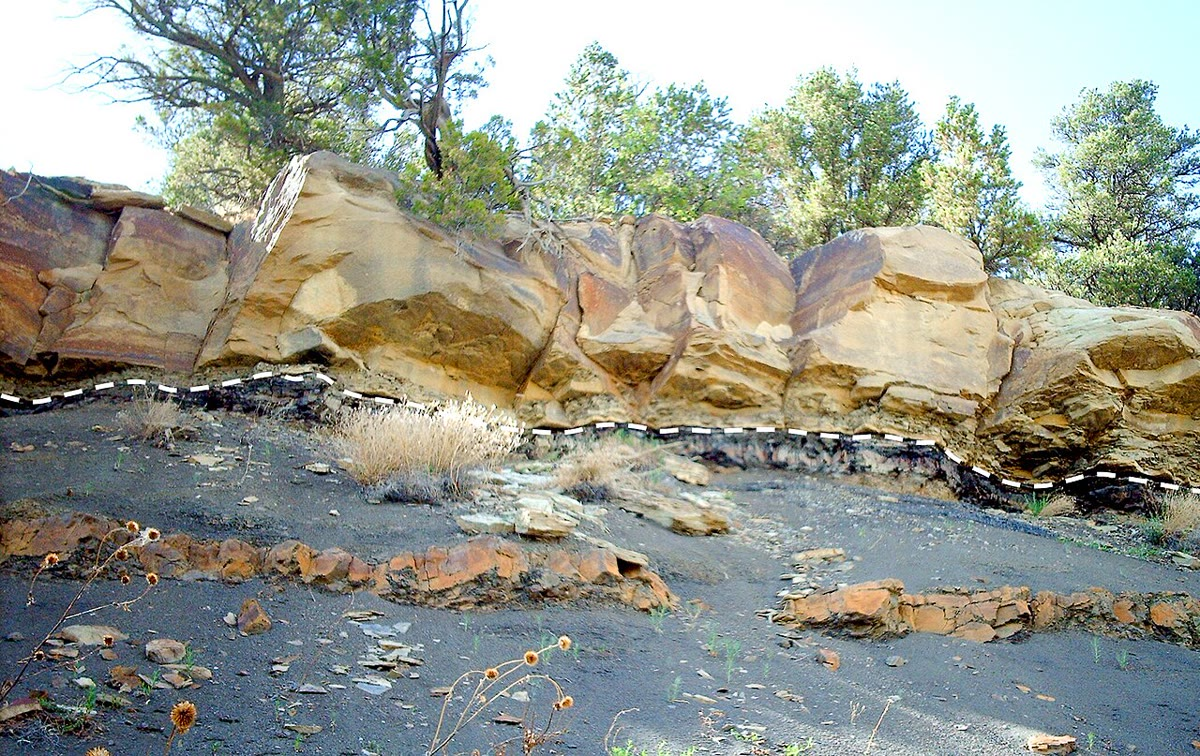
\includegraphics[width=0.78\linewidth]{images/book3/b1-kpg-boundary-trinidad.jpg}

{\small Batas antara Kapur dan Paleogen, ditandai oleh garis putus-putus, di Taman Negara Bagian Trinidad Lake, Colorado: batu pasir di atas, lapisan gelap di bawah dan sepanjang batas. (Nationalparks, CC~BY-SA~2.5, melalui Wikimedia Commons; garis putus-putus ada pada aslinya.)}
\label{fig:b1:stratigraphic-scale:kpg}
\end{omfigure}
% ledger: commons:kt-tlsp

\subsection*{Akhir Perm}

Kepunahan di akhir Perm adalah kehilangan kehidupan laut dan darat yang paling parah dalam setengah miliar tahun terakhir. Di Meishan di Tiongkok, penampang yang memuat GSSP dasar Trias, lima lapisan abu telah ditanggal dengan metode uranium--timbal pada zirkon. Mereka menempatkan kepunahan antara \qty[uncertainty-mode=separate]{251.941(37)}{\Ma} dan \qty[uncertainty-mode=separate]{251.880(31)}{\Ma}: interval \num[uncertainty-mode=separate]{60 \pm 48} ribu tahun. Penurunan negatif tajam sebesar \qty{3}{\permil} pada isotop karbon dari karbonat mendahuluinya, dan siklus karbon tetap tidak stabil selama sekitar \num{500} ribu tahun.
% ledger: burgess:end-permian, gssp:induan

Dasar Trias sendiri, \qty[uncertainty-mode=separate]{251.902(24)}{\Ma}, tidak ditempatkan pada kepunahan melainkan pada kemunculan pertama konodont \emph{Hindeodus parvus}, sebuah level yang jatuh di dalam interval kepunahan yang diberi tarikh di Meishan. Suatu kepunahan adalah sekumpulan kemunculan terakhir, yang diburamkan oleh pengawetan; satu kemunculan pertama dari spesies yang terkenal membuat garis yang lebih tajam. Penyebab kedua kepunahan itu --- sebuah tumbukan, provinsi basal besar --- menjadi pokok bahasan volume Tahun ke-2.
% ledger: gssp:induan, isg:biostratigraphy, burgess:end-permian

\section{Bagan internasional}\label{sec:b1:stratigraphic-scale:chart}

Bagan Kronostratigrafi Internasional menghimpun semua satuan, dari eonotem hingga \omterm{def:b1:stratigraphic-scale:chronostratigraphy}{tahap}, dalam satu tabel: nama-namanya, dasar setiap satuan dalam juta tahun dengan ketidakpastiannya, sebuah tanda untuk setiap dasar yang didefinisikan oleh GSSP yang telah disahkan, dan warna baku untuk setiap satuan, yaitu warna Komisi Peta Geologi Dunia. Bagian Fanerozoikum, yang direduksi menjadi era dan periodenya, digambar di bawah dari nilai-nilai bagan itu sendiri.
% ledger: ics:base.Paleozoic, ics:colour.Paleozoic, gssp:count

\begin{omfigure}
\begin{tikzpicture}[font=\footnotesize]
\begin{axis}[y dir=reverse, ymin=0, ymax=538.8, xmin=0, xmax=6.2,
  width=6.6cm, height=11cm, scale only axis, clip=false,
  axis x line=none, axis y line*=left, ytick={0,100,...,500},
  ylabel={umur (\unit{\Ma})}, tick label style={font=\scriptsize}]
  \pgfplotsinvokeforeach{Paleozoic,Mesozoic,Cenozoic,Cambrian,Ordovician,Silurian,Devonian,Carboniferous,Permian,Triassic,Jurassic,Cretaceous,Paleogene,Neogene,Quaternary}{
    \addplot[fill=ics#1, draw=black!70, line width=0.3pt] table[x=x, y=age] {figdata/out/bachelor-1-ics_chart-bar-#1.dat};}
  \node[rotate=90, font=\scriptsize\bfseries] at (axis cs:0.5,395.351) {Paleozoikum};
  \node[rotate=90, font=\scriptsize\bfseries] at (axis cs:0.5,158.951) {Mesozoikum};
  \node[rotate=90, font=\scriptsize\bfseries] at (axis cs:0.5,33) {Kenozoikum};
  \node[font=\scriptsize] at (axis cs:2,512.825) {Kambrium};
  \node[font=\scriptsize] at (axis cs:2,464.975) {Ordovisium};
  \node[font=\scriptsize] at (axis cs:2,431.36) {Silur};
  \node[font=\scriptsize] at (axis cs:2,389.24) {Devon};
  \node[font=\scriptsize] at (axis cs:2,328.88) {Karbon};
  \node[font=\scriptsize] at (axis cs:2,275.401) {Perm};
  \node[font=\scriptsize] at (axis cs:2,226.651) {Trias};
  \node[font=\scriptsize] at (axis cs:2,172.25) {Jura};
  \node[font=\scriptsize] at (axis cs:2,104.55) {Kapur};
  \node[font=\scriptsize] at (axis cs:2,44.52) {Paleogen};
  \node[font=\scriptsize] at (axis cs:2,12.81) {Neogen};
  \addplot[mark=-, mark size=3pt, only marks, nodes near coords, point meta=explicit symbolic,
    every node near coord/.style={anchor=west, xshift=1pt, font=\scriptsize}]
    table[x=x, y=age, meta=lab] {figdata/out/bachelor-1-ics_chart-bases.dat};
  \addplot[only marks, mark=triangle*, mark size=3pt, mark options={rotate=90, fill=omThm, draw=omThm}]
    table[x expr=\thisrow{x}+1.75, y=age] {figdata/out/bachelor-1-ics_chart-events.dat};
  \node[anchor=west, xshift=3pt, font=\scriptsize, text=omThm] at (axis cs:4.75,251.902) {akhir Perm};
  \node[anchor=west, xshift=3pt, font=\scriptsize, text=omThm] at (axis cs:4.75,66) {akhir Kapur};
  \node[anchor=south, font=\scriptsize] at (axis cs:2,0) {Kuarter};
  \node[anchor=west, font=\scriptsize] at (axis cs:3.0,-14) {0};
  \node[anchor=south, font=\scriptsize\itshape] at (axis cs:0.5,-30) {era};
  \node[anchor=south, font=\scriptsize\itshape] at (axis cs:2,-30) {periode};
  \node[anchor=south, font=\scriptsize\itshape] at (axis cs:3.5,-30) {dasar (\unit{\Ma})};
\end{axis}
\end{tikzpicture}

{\small Fanerozoikum pada bagan internasional: tiga era dan dua belas periodenya, dalam skala, dengan warna bagan, dan umur dasar setiap periode (ketidakpastian dihilangkan). Segitiga menandai dua dasar yang merupakan horizon kepunahan massal. Kuarter, sepanjang \qty{2.58}{\Ma}, adalah pita tipis di atas.}
\label{fig:b1:stratigraphic-scale:chart}
\end{omfigure}
% computed in figdata/bachelor-1/ics_chart.py; ledger: ics:base.Cambrian, ics:colour.Cambrian (every ics base and colour row of the eras and periods), burgess:end-permian, alvarez:iridium

Periode-periodenya sangat tidak sama (gambar di atas). Kapur berlangsung \qty{77.1}{\Ma}, Neogen \qty{20.46}{\Ma} dan Kuarter hanya \qty{2.58}{\Ma}; rerata dari dua belas adalah \qty{44.9}{\Ma}. Ketidaksamaan itu diwarisi: \omterm{def:b1:stratigraphic-scale:chronostratigraphy}{sistem-sistem} itu dinamai dalam klasifikasi awal, sebelum batuan mana pun ditanggal dalam tahun --- beberapa nama memberi posisi (Paleogen, Neogen, Kuarter), beberapa sebuah batuan (Karbon, Kapur), beberapa seorang suku bangsa atau sebuah tempat (Ordovisium, Silur, Devon, Perm) --- dan bagan tetap mempertahankan nama-nama itu sambil mendefinisikan dasarnya dengan GSSP. Umur dalam tahun berasal dari penanggalan isotop batuan vulkanik di dekat batas, seperti lapisan abu Meishan (\cref{ch:b1:radiometric-methods}), diinterpolasi seperti dalam \cref{prop:b1:stratigraphic-scale:interpolation}; versi baru bagan dapat menggeser suatu umur sementara GSSP tetap di tempatnya.
% ledger: ics:base.Cretaceous, ics:base.Neogene, ics:base.Quaternary, isg:chronostratigraphy, burgess:end-permian

\begin{dated}{2024}
% ledger: iugs:anthropocene
Antroposen, nama yang diusulkan pada 2001 untuk interval baru yang ditandai oleh aktivitas manusia, dipelajari sejak 2009 oleh kelompok kerja Subkomisi Stratigrafi Kuarter. Pada akhir 2023 kelompok itu mengusulkan suatu \omterm{def:b1:stratigraphic-scale:chronostratigraphy}{seri} yang dimulai sekitar 1950, dengan GSSP-nya dalam sedimen Danau Crawford, Ontario. Pemungutan suara subkomisi, yang ditutup pada 4 Maret 2024, menolaknya: 4 suara setuju, 12 menentang, 3 abstain, 3 anggota tidak memberi suara. Anggota pemberi suara Komisi Stratigrafi Internasional mengakui hasil pemungutan suara itu. Antroposen bukan satuan dalam bagan; ia tetap menjadi istilah tidak resmi, yang banyak dipakai.
\end{dated}

\section{Latihan}

\begin{exercise}[$\star$]\label{exo:b1:stratigraphic-scale:1}
Nyatakan apakah setiap nama adalah \omterm{def:b1:stratigraphic-scale:lithostratigraphy}{satuan litostratigrafi}, biostratigrafi, kronostratigrafi atau geokronologi, dan sebutkan peringkatnya jika punya: (a)~\omterm{def:b1:stratigraphic-scale:chronostratigraphy}{Sistem} Jura; (b)~\omterm{def:b1:stratigraphic-scale:lithostratigraphy}{Formasi} Serpih Mardon; (c)~Kapur Awal; (d)~Zona \emph{Hindeodus parvus}; (e)~\omterm{def:b1:stratigraphic-scale:chronostratigraphy}{Tahap} Danian; (f)~Epok Paleosen; (g)~sebuah \omterm{def:b1:stratigraphic-scale:lithostratigraphy}{anggota} batu pasir dari Serpih Mardon.
% ledger: isg:lithostratigraphy, isg:biostratigraphy, isg:chronostratigraphy
\end{exercise}

\begin{exercise}[$\star$]\label{exo:b1:stratigraphic-scale:2}
Dengan dasar era dalam gambar bagan (yaitu dasar Kambrium, Trias dan Paleogen), hitunglah durasi Paleozoikum, Mesozoikum dan Kenozoikum, dan bagian Fanerozoikum
yang masing-masing diwakilinya. Berapa bagian dari waktu sejak dasar Hadean, \qty{4567}{\Ma}, yang diwakili oleh seluruh Fanerozoikum?
% ledger: ics:base.Paleozoic, ics:base.Mesozoic, ics:base.Cenozoic, ics:base.Hadean
\end{exercise}

\begin{exercise}[$\star$]\label{exo:b1:stratigraphic-scale:3}
Sebuah tebing menunjukkan, dari bawah: lapisan A, B, C dan D, miring \ang{40}; sebuah dike E yang memotong A hingga D; sebuah permukaan erosi yang memotong puncak D dan dike; lapisan mendatar F dan G di atasnya; sebuah sesar yang menggeser A hingga F tetapi tidak G. Urutkan peristiwa-peristiwa itu, dan sebutkan prinsip yang membenarkan setiap langkah.
\end{exercise}

\begin{exercise}[$\star$]\label{exo:b1:stratigraphic-scale:4}
Dua lapisan abu berjarak \qty{30}{m} dalam serpih ditanggal \qty{85.40}{\Ma} (yang bawah) dan \qty{84.60}{\Ma} (yang atas). Kemunculan pertama \omterm{def:b1:stratigraphic-scale:biozone}{fosil indeks} terletak \qty{12}{m} di atas abu bawah. Hitunglah laju akumulasi dan umur kemunculan pertama itu, dengan asumsi laju konstan.
\end{exercise}

\begin{exercise}[$\star\star$]\label{exo:b1:stratigraphic-scale:5}
Dalam sebuah penampang, empat takson memiliki rentang (ketinggian dalam meter): A 0--34, B 12--50, C 26--62, D 41--70. (a)~Gambarlah diagram rentang. (b)~Berikan luas dan ketebalan \omterm{def:b1:stratigraphic-scale:biozone}{zona rentang} bersamaan dari B dan C, dan dari \omterm{def:b1:stratigraphic-scale:biozone}{zona interval} di antara kemunculan pertama B dan D. (c)~Di penampang kedua, B ditemukan dari 3 hingga 15~m dan C dari 9 hingga 22~m, dan tidak ada yang lain yang diketahui. Batas-batas zona dari (b) mana yang dapat dikenali di sana, dan mana yang tidak? Horizon mana yang dapat dikorelasikan antara kedua penampang dengan keyakinan paling besar?
\end{exercise}

\begin{exercise}[$\star\star$]\label{exo:b1:stratigraphic-scale:6}
Selama transgresi garis pantai bergerak ke pedalaman dengan \qty{20}{km} per juta tahun. (a)~Seberapa jauh umur puncak batu pasir garis pantai berbeda antara dua sumur yang berjarak \qty{60}{km} sepanjang arah transgresi? (b)~Sebuah abu jatuh satu juta tahun setelah garis pantai melewati sumur di sisi laut, tempat lumpur lepas pantai terakumulasi dengan \qty{30}{m} per juta tahun. Seberapa tinggi di atas puncak batu pasir lapisan abu itu ditemukan di sana? (c)~Di mana garis pantai ketika abu itu jatuh? Apakah abu ditemukan di atas atau di bawah batu pasir di sumur di sisi darat, dan mengapa ia mungkin tidak ditemukan di sana sama sekali? Jelaskan dengan sketsa.
\end{exercise}

\begin{exercise}[$\star\star$]\label{exo:b1:stratigraphic-scale:7}
(a)~Hitunglah ketidakpastian relatif umur dasar Lochkovium
(\qty[uncertainty-mode=separate]{419.62(136)}{\Ma}) dan Induan (\qty[uncertainty-mode=separate]{251.902(24)}{\Ma}), dalam persen. Usulkan mengapa keduanya berbeda jauh. (b)~Dari kedua umur yang mengapit kepunahan akhir Perm di Meishan,
\qty[uncertainty-mode=separate]{251.941(37)}{\Ma} dan
\qty[uncertainty-mode=separate]{251.880(31)}{\Ma}, hitunglah ulang durasi kepunahan dan ketidakpastiannya, dengan anggapan kedua kesalahan independen. Bandingkan dengan
\num[uncertainty-mode=separate]{60 \pm 48} ribu tahun yang diterbitkan.
% ledger: ics:base.Devonian, gssp:induan, burgess:end-permian
\end{exercise}

\begin{exercise}[$\star\star$]\label{exo:b1:stratigraphic-scale:8}
Ambil \omterm{def:b1:comparative-planetology:small-bodies}{asteroid} 1980 sebagai bola selebar \qty{10}{km}, bermassa jenis \qty{3000}{kg.m^{-3}} (nilai asumsi), yang melemparkan 60 kali massanya sebagai debu. (a)~Hitunglah massa \omterm{def:b1:comparative-planetology:small-bodies}{asteroid} dan debu. (b)~Sebarkan debu merata di atas Bumi (diameter \qty{12756}{km}): berapa massa yang jatuh pada setiap meter persegi? (c)~Diendapkan pada massa jenis \qty{2500}{kg.m^{-3}}, seberapa tebal lapisannya? (d)~Ulangi (c) untuk diameter \qty{6}{km} dan \qty{14}{km}, kisaran perkiraan itu. Bandingkan dengan ketebalan lempung batas di GSSP Danian.
% ledger: alvarez:iridium, planet:Earth.diameter, gssp:danian
\end{exercise}

\begin{exercise}[$\star\star$]\label{exo:b1:stratigraphic-scale:9}
(a)~Dalam penampang yang terkondensasi tempat sedimen terakumulasi pada \qty{2}{m} per juta tahun, berapa tebal interval \num{60} ribu tahun kepunahan akhir Perm? Berapa tebalnya untuk durasi terpendek dan terpanjang yang diizinkan oleh ketidakpastiannya? (b)~Dalam penampang laut dalam yang terakumulasi pada \qty{10}{m} per juta tahun, berapa tebal interval \num{32000} tahun tempat tumbukan dan batas K--Pg sinkron? (c)~Apa yang dikatakan angka-angka ini tentang pengambilan sampel penampang untuk mempelajari kepunahan?
% ledger: burgess:end-permian, renne:kpg
\end{exercise}

\begin{exercise}[$\star\star\star$]\label{exo:b1:stratigraphic-scale:10}
Sebuah dataran pantai miring $1$ banding $2000$ dan \omterm{def:b1:diagenesis-basins:eustasy}{muka laut relatif} naik pada \qty{10}{m} per juta tahun. (a)~Dengan \cref{prop:b1:stratigraphic-scale:transgression}, seberapa cepat garis pantai bergerak ke pedalaman, dan seberapa jauh umur puncak batu pasir garis pantai berbeda antara dua sumur yang berjarak \qty{30}{km}? (b)~Sedimen kini dikirim ke pantai, yang membangun dataran pantai ke atas sebesar $a$ meter per juta tahun di garis pantai. Tunjukkan bahwa garis pantai bergerak ke pedalaman dengan $(R - a)/s$ selama $a < R$. Apa yang terjadi ketika $a > R$? (c)~Jelaskan mengapa puncak batu pasir yang umurnya berubah sebesar satu juta tahun dapat tampak, dalam satu tebing, persis seperti permukaan dengan umur sama.
\end{exercise}

\begin{exercise}[$\star\star\star$]\label{exo:b1:stratigraphic-scale:11}
Dua lapisan abu terletak pada \qty{10}{m} dan \qty{50}{m} dalam sebuah penampang dan ditanggal \qty[uncertainty-mode=separate]{100.50(5)}{\Ma} dan \qty[uncertainty-mode=separate]{99.70(3)}{\Ma}. (a)~Interpolasikan umur level pada \qty{25}{m} dan ketidakpastiannya dengan
\cref{prop:b1:stratigraphic-scale:interpolation}. (b)~Di mana di antara kedua abu ketidakpastiannya paling kecil? Carilah nilai $f$ yang meminimumkan $\sigma_t$, dan nilai minimumnya. (c)~Tunjukkan bahwa $\sigma_t$ tidak pernah melampaui yang lebih besar dari $\sigma_1$ dan $\sigma_2$ di antara kedua lapisan.
\end{exercise}

\begin{exercise}[$\star\star\star$]\label{exo:b1:stratigraphic-scale:12}
Sebuah sumur melewati serpih seragam. Sebuah abu yang ditanggal \qty{30.0}{\Ma} terletak pada kedalaman \qty{1000}{m} dan sebuah abu yang ditanggal \qty{29.0}{\Ma} pada \qty{200}{m}; sebuah batas \omterm{def:b1:stratigraphic-scale:chronostratigraphy}{tahap} terletak pada \qty{600}{m}. (a)~Interpolasikan umurnya dari kedalaman. (b)~Butirannya, bukan porinya, tiba dengan laju konstan. Dengan menggunakan serpih dari \cref{tab:b1:diagenesis-basins:athy} dan
\cref{prop:b1:diagenesis-basins:solid}, hitunglah ketebalan padat antara setiap abu dan batas, dan interpolasikan umur lagi secara proporsional terhadapnya. (c)~Berapa ribu tahun kedua perkiraan itu berbeda, dan mana yang lebih baik?
% ledger: pybacktrack:compaction
\end{exercise}

\section{Masalah: mengorelasikan tiga penampang melintasi sebuah cekungan}

\begin{problem}[{Soal akhir pekan --- bagaimana fosil, lapisan abu dan batu pasir yang diakronis bersama-sama menanggal batas sebuah tahap}]
\label{pb:b1:stratigraphic-scale:1}
% values: calc/ch24.py; the basin, its sections, its taxa (Vardenoceras and Ostreola) and its ash ages are invented
Tiga penampang dicatat sepanjang garis melintasi sebuah cekungan rekaan: A di barat, B \qty{25}{km} di timur A, dan C \qty{20}{km} di timur B. Di masing-masing, Batu Pasir Kell tertutup oleh Serpih Mardon. Ketinggian dalam meter di atas dasar setiap penampang:
\begin{center}
\small
\begin{tabular}{lccc}
\hline
 & A & B & C \\
\hline
ketebalan total yang dicatat & 80.0 & 66.0 & 32.0 \\
puncak Batu Pasir Kell & 45.0 & 20.0 & 6.0 \\
lapisan abu 1 (ditanggal \qty[uncertainty-mode=separate]{152.40(4)}{\Ma})       & 5.0  & 8.0  & 3.0 \\
lapisan abu 2 (ditanggal \qty[uncertainty-mode=separate]{151.20(4)}{\Ma})       & 71.0 & 56.0 & 27.0 \\
kemunculan pertama \emph{Vardenoceras medium} & 36.6 & 31.2 & 14.8 \\
kemunculan pertama \emph{Vardenoceras ultimum} & 65.8 & 52.0 & 24.8 \\
kemunculan terakhir \emph{Vardenoceras primum}   & 49.0 & 40.0 & 19.0 \\
\hline
\end{tabular}
\end{center}
\emph{V.~primum} ditemukan dari dasar setiap penampang. Kerang \emph{Ostreola} hanya ditemukan di Batu Pasir Kell, di ketiga penampang. Tiga \omterm{def:b1:stratigraphic-scale:biozone}{zona interval} didefinisikan: zona~1 hingga kemunculan pertama \emph{V.~medium}, zona~2 hingga kemunculan pertama \emph{V.~ultimum}, zona~3 di atasnya. Sebuah batas \omterm{def:b1:stratigraphic-scale:chronostratigraphy}{tahap} didefinisikan, pada GSSP-nya di tempat lain, oleh kemunculan pertama \emph{V.~medium}.

\medskip
\noindent\textbf{Bagian I --- Biozona.}
\begin{enumerate}
  \item Gambarlah ketiga penampang berdampingan dengan skala vertikal yang sama, dengan Batu Pasir Kell, lapisan abu dan batas zona.
  \item Berikan ketebalan zona~2 di setiap penampang, dan ketebalan bagian zona~3 yang tercatat.
  \item Mengapa dasar zona~1 tidak dapat diletakkan di salah satu dari ketiga penampang?
  \item Mengapa \emph{Ostreola} adalah \omterm{def:b1:stratigraphic-scale:biozone}{fosil indeks} yang buruk, betapapun umumnya ia?
  \item Di zona mana kemunculan terakhir \emph{V.~primum} jatuh di setiap penampang? Dapatkah ia berfungsi sebagai batas zona keempat?
  \item Korelasikan penampang-penampang dengan kemunculan pertama \emph{V.~medium} dan \emph{V.~ultimum}. Apa yang disarankan oleh rasio ketebalan zona~2?
\end{enumerate}

\noindent\textbf{Bagian II --- Batu Pasir Kell.}
\begin{enumerate}[resume]
  \item Di zona mana puncak Batu Pasir Kell berada di setiap penampang?
  \item Apakah puncak Batu Pasir Kell merupakan permukaan dengan umur sama? Ke arah mana garis pantai bergerak, dan jenis peristiwa apa ini?
  \item Lapisan abu~1 berada di Batu Pasir Kell di ketiga penampang, lapisan abu~2 di Serpih Mardon. Mengapa lapisan abu lebih baik sebagai garis waktu daripada batas \omterm{def:b1:stratigraphic-scale:lithostratigraphy}{formasi}?
  \item Yang mana dari prinsip-prinsip dalam \cref{def:b1:stratigraphic-scale:principles} membenarkan mengikuti satu lapisan abu dari A hingga C?
\end{enumerate}

\noindent\textbf{Bagian III --- Laju.}
\begin{enumerate}[resume]
  \item Hitunglah laju akumulasi antara kedua lapisan abu di setiap penampang, dalam meter per juta tahun.
  \item Usulkan mengapa laju turun dari A ke C.
  \item Berapa tahun yang diwakili oleh sampel setebal \qty{10}{cm} di setiap penampang? Penampang mana yang memberi resolusi waktu paling halus?
  \item Dengan menganggap laju konstan, hitunglah umur puncak Batu Pasir Kell di setiap penampang.
  \item Hitunglah kecepatan garis pantai antara C dan B dan antara B dan A, dalam kilometer per juta tahun. Apakah transgresi bertambah cepat atau melambat?
  \item Hitunglah umur kemunculan pertama \emph{V.~ultimum} di setiap penampang.
  \item Apakah ketiga umur pada soal 16 sepakat dalam ketidakpastian penanggalan abu? Apa artinya ini bagi kemunculan pertama?
\end{enumerate}

\noindent\textbf{Bagian IV --- Umur batas.}
\begin{enumerate}[resume]
  \item Interpolasikan, di setiap penampang, umur kemunculan pertama \emph{V.~medium}.
  \item Hitunglah ketidakpastian setiap umur dari ketidakpastian penanggalan abu dengan \cref{prop:b1:stratigraphic-scale:interpolation}.
  \item Hitunglah rerata ketiga umur dan sebarannya. Apakah sebarannya lebih besar atau lebih kecil daripada ketidakpastian pada soal 19?
  \item Di penampang A kemunculan pertama \emph{V.~medium} terletak di Batu Pasir Kell, di B dan C di Serpih Mardon. Bagaimana perubahan litologi di antara lapisan abu dapat membiaskan interpolasi di A?
  \item Penampang mana dari ketiganya akan menjadi \omterm{def:b1:stratigraphic-scale:gssp}{stratotipe batas} terbaik, dan mengapa? Mana yang akan menjadi yang terburuk?
  \item Berapa lama zona~2 berlangsung?
  \item Berapa umur yang diinterpolasi dari batas itu?
\end{enumerate}
\end{problem}
